\documentclass[11pt,a4paper]{article}
\usepackage{float}
\usepackage{verbatim}
\usepackage{subfig}
\usepackage[T1]{fontenc}
\usepackage[utf8]{inputenc}
\usepackage{geometry}
\geometry{verbose,lmargin=2cm,rmargin=2cm, bmargin=3cm, tmargin=3cm}
\usepackage{enumitem}
\usepackage{wrapfig}
\usepackage{tikz}
\usetikzlibrary{decorations.markings}
\usepackage{calc}
\usepackage{wrapfig}
\usepackage{graphicx}
\usepackage{amssymb}
\usepackage{amsmath}
\usepackage{esint}
\usepackage{blindtext}
\usepackage{hyperref}
\usepackage{listings}

\hypersetup{
    colorlinks=true,
    linkcolor=blue,
    filecolor=magenta,
    urlcolor=cyan,
}
\usepackage{listings}
\lstset{ %
  backgroundcolor=\color{white},   % choose the background color; you must add \usepackage{color} or \usepackage{xcolor}; should come as last argument
  basicstyle=\footnotesize,        % the size of the fonts that are used for the code
  breakatwhitespace=false,         % sets if automatic breaks should only happen at whitespace
  breaklines=true,                 % sets automatic line breaking
  captionpos=t,                    % sets the caption-position to bottom
  commentstyle=\color{teal},    % comment style
  deletekeywords={...},            % if you want to delete keywords from the given language
  escapeinside={\%*}{*)},          % if you want to add LaTeX within your code
  extendedchars=true,              % lets you use non-ASCII characters; for 8-bits encodings only, does not work with UTF-8
  frame=single,                    % adds a frame around the code
  keepspaces=true,                 % keeps spaces in text, useful for keeping indentation of code (possibly needs columns=flexible)
  keywordstyle=\color{blue},       % keyword style
 % language=Python,                 % the language of the code
  morekeywords={*,...},           % if you want to add more keywords to the set
  numbers=left,                    % where to put the line-numbers; possible values are (none, left, right)
  numbersep=5pt,                   % how far the line-numbers are from the code
  numberstyle=\tiny\color{black}, % the style that is used for the line-numbers
  rulecolor=\color{black},         % if not set, the frame-color may be changed on line-breaks within not-black text (e.g. comments (green here))
  showspaces=false,                % show spaces everywhere adding particular underscores; it overrides 'showstringspaces'
  showstringspaces=false,          % underline spaces within strings only
  showtabs=false,                  % show tabs within strings adding particular underscores
  stepnumber=1,                    % the step between two line-numbers. If it's 1, each line will be numbered
  tabsize=2,                       % sets default tabsize to 2 spaces
  title=\lstname                   % show the filename of files included with \lstinputlisting; also try caption instead of title
}
\begin{document}

\title{Polarization\\
\normalsize{FYS2150 Lab Report}\\}

\author{Nicholas Karlsen}
% \email{nichoka@student.matnat.uio.no}

\date{\today}% It is always \today, today,
%  but any date may be explicitly specified

\maketitle
\begin{abstract}
  Studying the properties of linearly and circularly polarized light and testing how well the properties match up to theoretical predictions.
\end{abstract}

\twocolumn

%\tableofcontents

\section{\label{sect:intro}Introduction}
  

\section{\label{sect:theory}Theory}

\section{\label{section:experimental}Experimental Procedure} 
  
  In order to minimize the effects that ambient light may have on the following experiments, the windows in the room were covered up and all lights not related to the experiment were turned off whilst data was being recorded, or observations were made.

  \subsection{Checking the polarization of the spectral lamp}
    In order to determine whether or not the light emitted from a speciffic Sodium spectral lamp, the intensity of light was measured using a luxmeter after having gone through a polarization filter of variable angle acting as an analyzator, depicted in Fig \ref{fig:lux_ana_lamp}. When changing the angle of the analyzator, we defined a positive and negative direction, which was kept for all subsequent measurements using polarization filters. The angle of the polarization filter was changed in $10^\circ$ increments in the range $-90^\circ$ to $90^\circ$ and the intensity of the light measured by the luxmeter was noted for each angle. 


  \begin{figure}[H]
    \center
    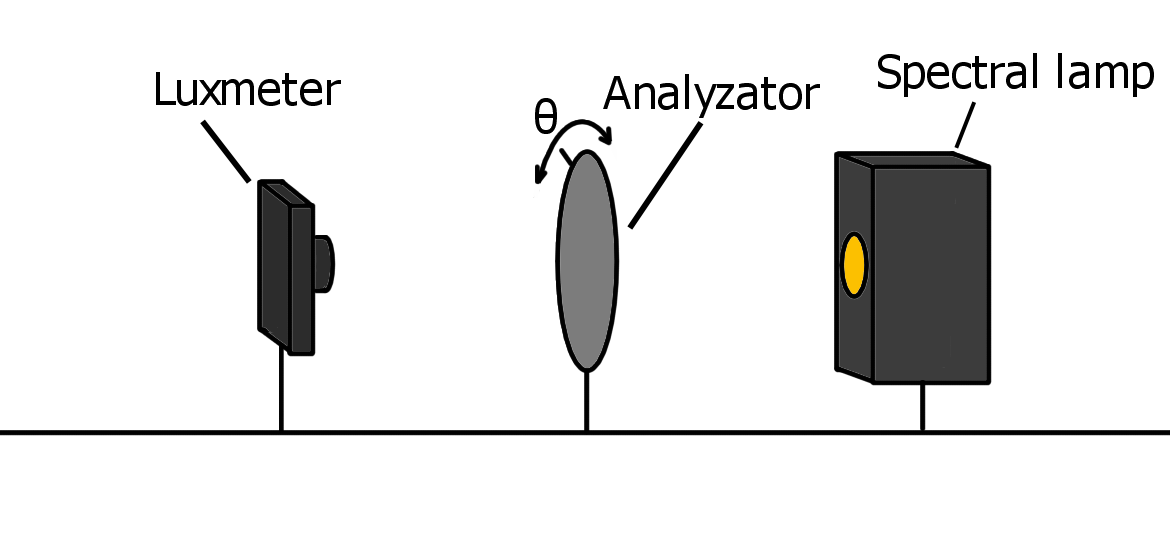
\includegraphics[width=8cm]{scripts/figs/diagram_1.png}
    \caption{Aparature to test the polarization of light emitted from a spectral lamp using a polarization filter with variable angle $\theta$ as an analyzator and measuring the intensity of the filtered light using the luxmeter.}
    \label{fig:lux_ana_lamp}
  \end{figure}

  \subsection{Testing Malus' law}


    \begin{figure}[H]
      \center
      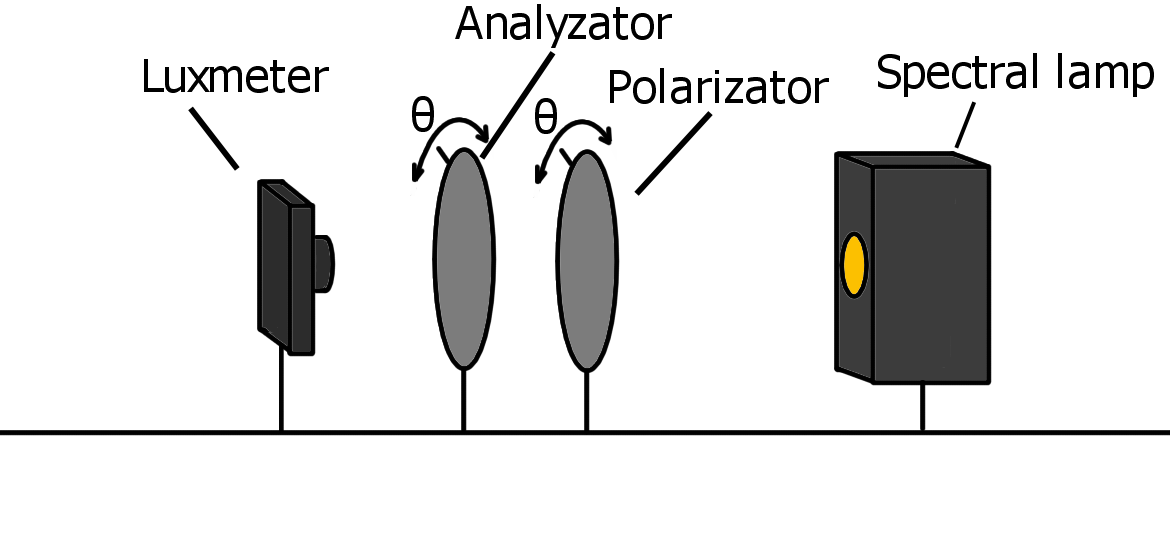
\includegraphics[width=8cm]{scripts/figs/diagram_2.png}
      \caption{Aparature to test Malus' law.}
      \label{fig:lux_ana_pola_lamp}
    \end{figure}


\section{\label{sect:results}Results}
  
  The intensity measurements presented in table \ref{tab:ana}, where light from a spectral lamp is passed through a single polarization filter has a standard deviation of 19, which is used as the estimated uncertainty for further measurements made with the luxmeter.


  \begin{table}[H]
      \center
      \caption{Measured intensity when passing unpolarized light through a single polarization filter, $\theta$ denoting the angle of the filter. Aparature depicted in Fig. \ref{fig:lux_ana_lamp}}
       \begin{tabular}{r | l}
        $\theta$ [deg] & Intensity [Lux] \\ \hline
         \input{scripts/data/ana.dat}
       \end{tabular}
       \label{tab:ana}
  \end{table}



  \begin{figure}[H]
    \center
    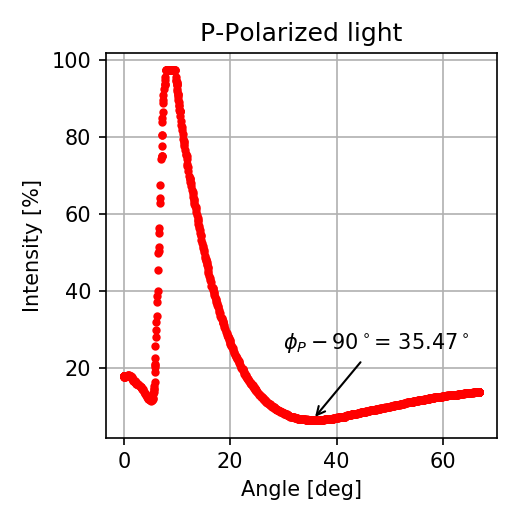
\includegraphics[width=8cm]{scripts/ppolar.png}
    \caption{Intensity profile due to p-polarized light, where $\phi_P$ denotes the Brewster angle.}
  \end{figure}

  \begin{figure}[H]
    \center
    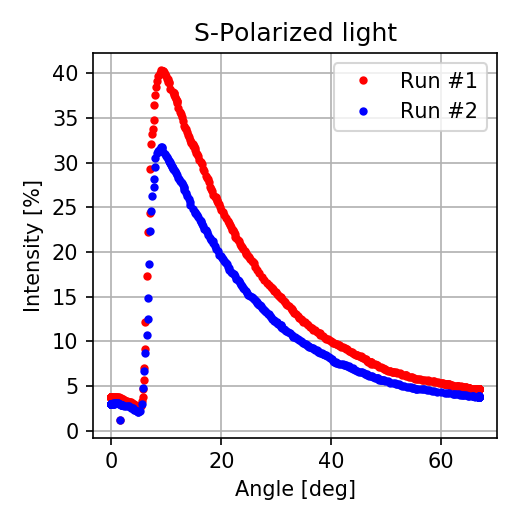
\includegraphics[width=8cm]{scripts/spolar.png}
    \caption{Intensity profile due to p-polarized light from two separate attempts of the experiment.}
  \end{figure}

\section{\label{sect:discuss}Discussion}

\section{\label{sect:conclusion}Conclusion}


\bibliographystyle{plain}
\bibliography{references.bib}

%%%%%%%%%%%%%%%%%%%%%%%%
%%% END OF MAIN BODY %%%
%%%%%%%%%%%%%%%%%%%%%%%%
\end{document}